\documentclass{standalone}
\usepackage{tikzstyle}
\usepackage{tabularx}
\begin{document}

\colorlet{c_lenses}{black}
\colorlet{c_ray}{red}

\begin{tabular}{*{4}{>{\centering\arraybackslash}m{0.2\textwidth}}}
%Gun
%
\begin{tikzpicture}[scale=0.3]
    \draw [pattern=north west lines] (-1, -1) -- ++ (1, 0) -- ++(0, 2) -- ++(-1, 0) -- ++(0, 0.5) -- ++(-0.5, 0) -- ++(0, -3) -- ++(0.5, 0) -- cycle;
\end{tikzpicture}
&
% Lense
%
\begin{tikzpicture}[scale=0.3]
    \filldraw [draw=c_lenses, fill=c_lenses!60, xshift=-1cm] (0, 2) rectangle ++(2, 2);
    \filldraw [draw=c_lenses, fill=c_lenses!60, xshift=-1cm] (0, -2) rectangle ++(2, -2);
    \filldraw[fill=c_lenses!10, draw=c_lenses] (-1, -2) rectangle ++(2, 4);
\end{tikzpicture}
&
%
%

\begin{tikzpicture}[scale=0.3]
    \filldraw [xshift=12cm] (-0.25, -2.5) rectangle ++(0.5, 5);
\end{tikzpicture}
&
%
%
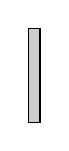
\begin{tikzpicture}[scale=0.3]
    \filldraw[fill=black!20, draw=black, xshift=16cm] (0, -2) rectangle (0.5, 2);
\end{tikzpicture}
\\
% Text
%
Source d'électrons&
Lentille électromagnétique&
Echantillon&
Détecteur\\
\end{tabular}

\end{document}